%% ============================================================
%% pynasonde — Comprehensive Methods & Capabilities Overview
%% Beamer presentation (compile with: make tutorials)
%%
%% Manual:
%%   cd tutorials/methods_ppt
%%   pdflatex pynasonde_methods_ppt.tex && pdflatex pynasonde_methods_ppt.tex
%%
%% Or via project root:
%%   make tutorials-methods
%% ============================================================
\documentclass[aspectratio=169,11pt]{beamer}

% ---------- theme ------------------------------------------------
\usetheme{Madrid}
\usecolortheme{crane}
\setbeamertemplate{navigation symbols}{}
\setbeamertemplate{footline}[frame number]
\setbeamerfont{frametitle}{size=\large,series=\bfseries}
\setbeamercolor{block title}{bg=blue!15,fg=blue!60!black}
\setbeamercolor{block body}{bg=blue!5}
\setbeamercolor{alertblock title}{bg=orange!25,fg=orange!70!black}
\setbeamercolor{alertblock body}{bg=orange!5}
\setbeamercolor{exampleblock title}{bg=green!15,fg=green!50!black}
\setbeamercolor{exampleblock body}{bg=green!5}

% ---------- packages ------------------------------------------------
\usepackage{amsmath,amssymb}
\usepackage{graphicx}
\usepackage{listings}
\usepackage{xcolor}
\usepackage{booktabs}
\usepackage{hyperref}
\usepackage{tikz}
\usepackage{multirow}
\usepackage{colortbl}
\usetikzlibrary{arrows.meta,positioning,shapes,fit,backgrounds}

% ---------- figure path ------------------------------------------------
\graphicspath{{../../docs/examples/figures/}}

% ---------- code style ------------------------------------------------
\definecolor{codebg}{RGB}{245,245,250}
\definecolor{codekw}{RGB}{0,0,180}
\definecolor{codestr}{RGB}{160,32,32}
\definecolor{codecom}{RGB}{0,128,0}

\lstset{
  language=Python,
  backgroundcolor=\color{codebg},
  basicstyle=\ttfamily\scriptsize,
  keywordstyle=\color{codekw}\bfseries,
  stringstyle=\color{codestr},
  commentstyle=\color{codecom}\itshape,
  showstringspaces=false,
  breaklines=true,
  frame=single,
  framerule=0.4pt,
  rulecolor=\color{gray!40},
  xleftmargin=4pt,xrightmargin=4pt,
}

% ---------- handy command for figure sizing ----------------------
\newcommand{\figlw}[2]{\includegraphics[width=#1\linewidth,keepaspectratio]{#2}}

% ---------- title info -----------------------------------------------
\title[pynasonde — Methods \& Capabilities]{%
  \textbf{pynasonde} — Methods \& Capabilities Overview}
\subtitle{An open-source Python library for ionosonde data processing\\
  \small\normalfont Chakraborty et al., \textit{SoftwareX} 34, 102617 (2026)}
\author{S. Chakraborty \and T. Bullett \and A. Barjatya \and J. Mabie}
\institute{Embry-Riddle Aeronautical University \;|\; Fourth State Communications}
\date{\today}

% =================================================================
\begin{document}
% =================================================================

\begin{frame}
  \titlepage
  \vspace{-0.6cm}
  \begin{center}
    \small
    \texttt{pip install pynasonde}\quad|\quad
    \href{https://github.com/shibaji7/pynasonde}{github.com/shibaji7/pynasonde}\quad|\quad
    \href{https://pynasonde.readthedocs.io}{pynasonde.readthedocs.io}
  \end{center}
\end{frame}

\begin{frame}{Outline}
  \tableofcontents
\end{frame}

% ================================================================
\section{What is pynasonde?}
% ================================================================

\begin{frame}{Why pynasonde?}
\begin{columns}
\column{0.56\textwidth}
  \begin{itemize}\small
    \item \textbf{Problem}: Digisonde tools (Java) and VIPIR tools are
          instrument-specific, fragmented, and not always publicly available
    \item \textbf{Solution}: A unified, open-source Python framework for
          \emph{both} instrument families
    \item \textbf{Key design goals}:
      \begin{itemize}\scriptsize
        \item Modular architecture (read $\to$ plot $\to$ analyse)
        \item Support 9 file formats (binary + ASCII + XML)
        \item Lower barrier to reproducible analysis
        \item Built-in analysis pipeline, not just plotting
      \end{itemize}
    \item \textbf{Published}: Chakraborty et al., \textit{SoftwareX} 34, 102617 (2026)
    \item \textbf{Current}: v1.0 — substantially extended beyond publication
  \end{itemize}
\column{0.41\textwidth}
  \begin{block}{Installed capabilities}
    \scriptsize
    \textbf{9 file formats} read\\
    \textbf{7 digisonde} parsers\\
    \textbf{6 VIPIR} I/O classes\\
    \textbf{9 analysis} modules\\
    \textbf{20+} public API classes\\
    \textbf{Full pipeline} automation
  \end{block}
  \begin{alertblock}{Cite as}
    \tiny
    Chakraborty et al.\ (2026).\\
    \textit{SoftwareX} 34, 102617.\\
    DOI: 10.1016/j.softx.2026.102617\\
    Zenodo: 10.5281/zenodo.17476077
  \end{alertblock}
\end{columns}
\end{frame}

% ================================================================
\section{Architecture}
% ================================================================

%% ---- v1.0 published architecture ----
\begin{frame}{pynasonde v1.0 Architecture (Chakraborty et al.\ 2026)}
\vspace{-0.2cm}
\begin{center}
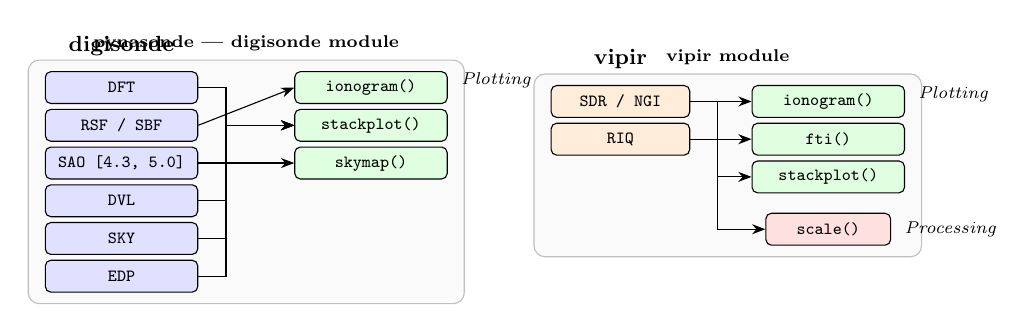
\begin{tikzpicture}[
  >=Stealth,
  every node/.style={font=\scriptsize},
  dnode/.style={draw,fill=blue!12,rounded corners=2pt,
                minimum width=2.2cm,minimum height=0.46cm,align=center},
  vnode/.style={draw,fill=orange!15,rounded corners=2pt,
                minimum width=2.0cm,minimum height=0.46cm,align=center},
  pnode/.style={draw,fill=green!12,rounded corners=2pt,
                minimum width=2.2cm,minimum height=0.46cm,align=center},
  snode/.style={draw,fill=red!12,rounded corners=2pt,
                minimum width=1.8cm,minimum height=0.46cm,align=center},
  scale=0.88,transform shape
]

% ---- DIGISONDE data types (left column) ----
\node[dnode] (dft) at (0,0)    {\texttt{DFT}};
\node[dnode,below=2pt of dft]  (rsf)  {\texttt{RSF / SBF}};
\node[dnode,below=2pt of rsf]  (sao)  {\texttt{SAO [4.3, 5.0]}};
\node[dnode,below=2pt of sao]  (dvl)  {\texttt{DVL}};
\node[dnode,below=2pt of dvl]  (sky)  {\texttt{SKY}};
\node[dnode,below=2pt of sky]  (edp)  {\texttt{EDP}};

% ---- DIGISONDE plotting methods ----
\node[pnode] (iono)  at (3.6,0)   {\texttt{ionogram()}};
\node[pnode,below=2pt of iono]  (stack) {\texttt{stackplot()}};
\node[pnode,below=2pt of stack] (skmap) {\texttt{skymap()}};

% digisonde arrows
\draw[->] (rsf.east)  -- (iono.west);
\draw[->] (sao.east)  -| ++(0.4,0) |- (stack.west);
\draw[->] (dft.east)  -| ++(0.4,0) |- (stack.west);
\draw[->] (dvl.east)  -| ++(0.4,0) |- (stack.west);
\draw[->] (sky.east)  -| ++(0.4,0) |- (skmap.west);
\draw[->] (edp.east)  -| ++(0.4,0) |- (stack.west);

% ---- VIPIR data types ----
\node[vnode] (sdr) at (7.2, -0.2)  {\texttt{SDR / NGI}};
\node[vnode,below=2pt of sdr] (riq) {\texttt{RIQ}};

% ---- VIPIR plotting methods ----
\node[pnode] (viono)  at (10.2,-0.2) {\texttt{ionogram()}};
\node[pnode,below=2pt of viono]  (fti)    {\texttt{fti()}};
\node[pnode,below=2pt of fti]    (vstack) {\texttt{stackplot()}};

% VIPIR processing
\node[snode,below=8pt of vstack] (scale)  {\texttt{scale()}};

% VIPIR arrows
\draw[->] (sdr.east) -- ++(0.4,0) |- (viono.west);
\draw[->] (sdr.east) -- ++(0.4,0) |- (fti.west);
\draw[->] (riq.east) -- ++(0.4,0) |- (vstack.west);
\draw[->] (riq.east) -- ++(0.4,0) |- (scale.west);

% ---- Module labels ----
\node[font=\bfseries\small,above=3pt of dft] {digisonde};
\node[font=\bfseries\small,above=3pt of sdr] {vipir};
\node[font=\scriptsize\itshape,right=2pt of iono,yshift=3pt]  {Plotting};
\node[font=\scriptsize\itshape,right=2pt of viono,yshift=3pt] {Plotting};
\node[font=\scriptsize\itshape,right=2pt of scale]            {Processing};

% ---- Outer pynasonde box ----
\begin{pgfonlayer}{background}
  \node[draw=gray!50,rounded corners=4pt,fill=gray!4,
        fit=(dft)(edp)(iono)(skmap),
        inner xsep=6pt,inner ysep=4pt,label=above:{\bfseries pynasonde — digisonde module}] {};
  \node[draw=gray!50,rounded corners=4pt,fill=gray!4,
        fit=(sdr)(riq)(viono)(scale),
        inner xsep=6pt,inner ysep=4pt,label=above:{\bfseries vipir module}] {};
\end{pgfonlayer}

\end{tikzpicture}
\end{center}
\vspace{0.1cm}
{\scriptsize Adapted from Fig.~2 of Chakraborty et al.\ (2026), \textit{SoftwareX} 34, 102617.}
\end{frame}

%% ---- Extended architecture (post-v1.0) ----
\begin{frame}{Extended Architecture — Post-v1.0 Additions}
\vspace{-0.1cm}
\begin{center}
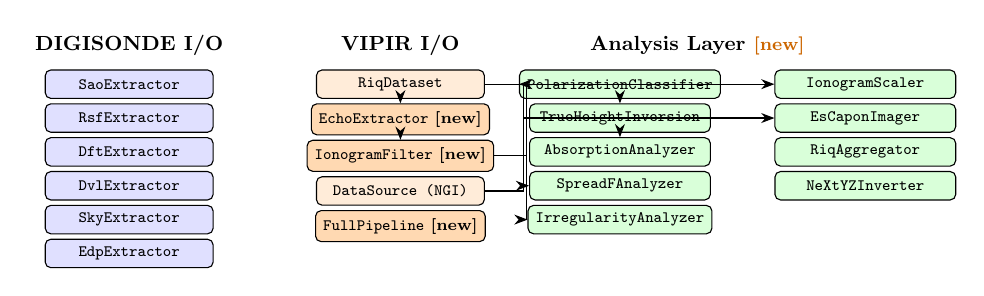
\begin{tikzpicture}[
  >=Stealth,
  every node/.style={font=\scriptsize},
  ioD/.style={draw,fill=blue!12,rounded corners=2pt,
              minimum width=2.6cm,minimum height=0.44cm,align=center},
  ioV/.style={draw,fill=orange!15,rounded corners=2pt,
              minimum width=2.6cm,minimum height=0.44cm,align=center},
  newV/.style={draw,fill=orange!30,rounded corners=2pt,
               minimum width=2.6cm,minimum height=0.44cm,align=center},
  an/.style={draw,fill=green!15,rounded corners=2pt,
             minimum width=2.8cm,minimum height=0.44cm,align=center},
  hdr/.style={font=\bfseries\small},
  scale=0.82,transform shape
]

%% Row 0: headers
\node[hdr] (hD) at (-4.2,2.4)  {DIGISONDE I/O};
\node[hdr] (hV) at ( 0.0,2.4)  {VIPIR I/O};
\node[hdr] (hA) at ( 4.6,2.4)  {Analysis Layer {\footnotesize\color{orange!80!black}[new]}};

%% DIGISONDE I/O column
\node[ioD] (sao)  at (-4.2, 1.8) {\texttt{SaoExtractor}};
\node[ioD,below=2pt of sao]  (rsf) {\texttt{RsfExtractor}};
\node[ioD,below=2pt of rsf]  (dft) {\texttt{DftExtractor}};
\node[ioD,below=2pt of dft]  (dvl) {\texttt{DvlExtractor}};
\node[ioD,below=2pt of dvl]  (sky) {\texttt{SkyExtractor}};
\node[ioD,below=2pt of sky]  (edp) {\texttt{EdpExtractor}};

%% VIPIR I/O column
\node[ioV] (riq)  at (0.0, 1.8)  {\texttt{RiqDataset}};
\node[newV,below=2pt of riq]  (echo) {\texttt{EchoExtractor} \textbf{[new]}};
\node[newV,below=2pt of echo] (filt) {\texttt{IonogramFilter} \textbf{[new]}};
\node[ioV,below=2pt of filt]  (ngi)  {\texttt{DataSource (NGI)}};
\node[newV,below=2pt of ngi]  (pipe) {\texttt{FullPipeline} \textbf{[new]}};

%% Analysis layer — two sub-columns
\node[an] (pol)  at (3.4, 1.8)  {\texttt{PolarizationClassifier}};
\node[an,below=2pt of pol]  (inv)  {\texttt{TrueHeightInversion}};
\node[an,below=2pt of inv]  (abs)  {\texttt{AbsorptionAnalyzer}};
\node[an,below=2pt of abs]  (sf)   {\texttt{SpreadFAnalyzer}};
\node[an,below=2pt of sf]   (irr)  {\texttt{IrregularityAnalyzer}};

\node[an] (scl) at (7.2, 1.8)  {\texttt{IonogramScaler}};
\node[an,below=2pt of scl]  (es)   {\texttt{EsCaponImager}};
\node[an,below=2pt of es]   (agg)  {\texttt{RiqAggregator}};
\node[an,below=2pt of agg]  (nxt)  {\texttt{NeXtYZInverter}};

%% Arrows: VIPIR processing chain
\draw[->] (riq.south)  -- (echo.north);
\draw[->] (echo.south) -- (filt.north);
\draw[->] (filt.east)  -- ++(0.5,0) |- (pol.west);
\draw[->] (filt.east)  -- ++(0.5,0) |- (sf.west);
\draw[->] (filt.east)  -- ++(0.5,0) |- (irr.west);
\draw[->] (pol.south)  -- (inv.north);
\draw[->] (inv.south)  -- (abs.north);
\draw[->] (riq.east)   -- ++(0.6,0) |- (es.west);
\draw[->] (ngi.east)   -- ++(0.6,0) |- (scl.west);

\end{tikzpicture}
\end{center}
\vspace{0.1cm}
{\scriptsize Orange = new since publication.\ \ Green = analysis layer (entirely new post-v1.0).}
\end{frame}

% ================================================================
\section{DIGISONDE Module}
% ================================================================

\begin{frame}{DIGISONDE Module — File Formats \& Parsers}
\vspace{-0.1cm}
\begin{center}
\scriptsize
\begin{tabular}{lll>{\raggedright\arraybackslash}p{5.0cm}}
  \toprule
  \textbf{Ext.} & \textbf{Type} & \textbf{Parser class} & \textbf{Key methods / output} \\
  \midrule
  \texttt{.SAO 4.3} & ASCII  & \texttt{SaoExtractor}  & \texttt{load\_SAO\_files()}: \texttt{height\_profile} / \texttt{scaled\_params} \\
  \texttt{.SAO 5.0} & XML    & \texttt{SaoExtractor}  & same API; \texttt{SaoSummaryPlots.plot\_TS()} \\
  \texttt{.RSF}     & Binary & \texttt{RsfExtractor}  & \texttt{plot\_direction\_ionogram()}, \texttt{plot\_directogram()} \\
  \texttt{.SBF}     & Binary & \texttt{SbfExtractor}  & \texttt{extract()}, \texttt{ionogram()} \\
  \texttt{.DFT}     & ASCII  & \texttt{DftExtractor}  & \texttt{plot\_doppler\_waterfall()}, \texttt{plot\_doppler\_spectra()} \\
  \texttt{.DVL}     & ASCII  & \texttt{DvlExtractor}  & \texttt{load\_DVL\_files()}, \texttt{plot\_dvl\_drift\_velocities()} \\
  \texttt{.SKY}     & ASCII  & \texttt{SkyExtractor}  & \texttt{extract()}, \texttt{to\_pandas()}, \texttt{plot\_skymap()} \\
  \texttt{.EDP}     & ASCII  & \texttt{EdpExtractor}  & \texttt{extract()}, electron density profile \\
  \bottomrule
\end{tabular}
\end{center}
\vspace{0.15cm}
\begin{columns}
\column{0.50\textwidth}
  \begin{block}{\small Parallel loading}
    \scriptsize
    \texttt{SaoExtractor.load\_SAO\_files(folders, n\_procs=4)}\\
    \texttt{DvlExtractor.load\_DVL\_files(folder, n\_procs=4)}
  \end{block}
\column{0.47\textwidth}
  \begin{alertblock}{\small New post-v1.0}
    \scriptsize
    DFT waterfall, RSF direction-coded ionogram + directogram,
    multi-panel SKY sequence
  \end{alertblock}
\end{columns}
\end{frame}

\begin{frame}[fragile]{DIGISONDE — SAO: Density Profiles \& Scaled Parameters}
\begin{columns}
\column{0.52\textwidth}
  \begin{lstlisting}
from pynasonde.digisonde.parsers.sao \
    import SaoExtractor, SaoSummaryPlots

# N(h) profiles for a whole day
df = SaoExtractor.load_SAO_files(
    folders=["data/KR835/"],
    func_name="height_profile",
    n_procs=4,
)
# cols: datetime, height_km,
#       plasma_freq_mhz, Ne_cm3

# Scaled ionospheric parameters
params = SaoExtractor.load_SAO_files(
    folders=["data/KR835/"],
    func_name="scaled_params",
)
# cols: datetime, foF2, hmF2, foE, MUF

SaoSummaryPlots(df).plot_TS(
    params=["foF2","hmF2"])
  \end{lstlisting}
\column{0.44\textwidth}
  \begin{center}
    \figlw{0.96}{sao_isodensity_KR835.png}\\[3pt]
    {\scriptsize Daily isodensity contour, KR835.}
  \end{center}
\end{columns}
\end{frame}

\begin{frame}[fragile]{DIGISONDE — RSF: Direction-Coded Ionogram}
\vspace{-0.2cm}
\begin{columns}[T]
\column{0.42\textwidth}
  \begin{lstlisting}
from pynasonde.digisonde.parsers.rsf \
    import RsfExtractor

ex = RsfExtractor("KR835.RSF")
ex.extract()

# colour-coded by arrival azimuth
ex.plot_direction_ionogram()

# full day: TID / ground distance
ex.plot_directogram()
  \end{lstlisting}
  \vspace{0.1cm}
  \begin{block}{\scriptsize What RSF adds}
    \scriptsize
    \begin{itemize}\setlength{\itemsep}{0pt}
      \item Arrival azimuth per echo (4 Rx)
      \item Full amplitude + phase
      \item Directogram = TID signature
    \end{itemize}
  \end{block}
\column{0.27\textwidth}
  \begin{center}
    \figlw{0.99}{rsf_direction_ionogram_KR835.png}
    {\scriptsize Direction ionogram}
  \end{center}
\column{0.27\textwidth}
  \begin{center}
    \figlw{0.99}{rsf_directogram_KR835_daily.png}
    {\scriptsize Directogram (daily)}
  \end{center}
\end{columns}
\end{frame}

\begin{frame}[fragile]{DIGISONDE — DFT, DVL, SKY}
\vspace{-0.25cm}
\begin{columns}[T]
\column{0.49\textwidth}
  \begin{lstlisting}[title={DFT}]
dft = DftExtractor("KR835.DFT")
dft.extract()
dft.plot_doppler_waterfall()
  \end{lstlisting}
  \vspace{2pt}
  \begin{lstlisting}[title={DVL}]
dvl = DvlExtractor.load_DVL_files(
    folder="data/KR835/", n_procs=4)
dvl.plot_dvl_drift_velocities()
# panels: Vx(E), Vy(N), Vz(up)
  \end{lstlisting}
  \vspace{2pt}
  \begin{lstlisting}[title={SKY}]
sky = SkyExtractor("KR835.SKY")
sky.extract()
SkySummaryPlots(sky.to_pandas())\
    .plot_skymap()
  \end{lstlisting}
\column{0.48\textwidth}
  \begin{center}
    \figlw{0.88}{stackplots_dvl.png}
  \end{center}
\end{columns}
\end{frame}

% ================================================================
\section{VIPIR Module}
% ================================================================

\begin{frame}{VIPIR Module — File Formats \& I/O Classes}
\vspace{-0.1cm}
\begin{center}
\scriptsize
\begin{tabular}{lll>{\raggedright\arraybackslash}p{5.2cm}}
  \toprule
  \textbf{Ext.} & \textbf{Type} & \textbf{I/O class} & \textbf{Key methods} \\
  \midrule
  \texttt{.RIQ} & Binary & \texttt{RiqDataset} &
    \texttt{create\_from\_file()}, SCT + PCT, \texttt{VIPIR\_VERSION\_MAP} \\
  \texttt{.RIQ} & — & \texttt{EchoExtractor} \textbf{[new]} &
    7-param echoes (h, A, V*, EP, PP, XL, YL); \texttt{to\_dataframe()} \\
  \texttt{.RIQ} & — & \texttt{IonogramFilter} \textbf{[new]} &
    6-stage: RFI, EP, multi-hop, DBSCAN, RANSAC, temporal \\
  \texttt{.NGI} & NetCDF & \texttt{DataSource} &
    \texttt{load()}, multi-SDR data cube aggregation \\
  \texttt{.NGI} & — & \texttt{AutoScaler} &
    noise profile, segmentation, binary trace extraction \\
  \texttt{.RIQ} & — & \texttt{FullPipeline} \textbf{[new]} &
    end-to-end: RIQ $\to$ echoes $\to$ filter $\to$ O/X $\to$ N(h) \\
  \bottomrule
\end{tabular}
\end{center}
\vspace{0.15cm}
\begin{columns}
\column{0.50\textwidth}
  \begin{block}{\small Supported stations}
    \scriptsize
    WI937 — Wallops Island (data\_type=1)\\
    PL407 — Prudhoe Bay (data\_type=2)\\
    Generic via \texttt{VIPIR\_VERSION\_MAP}
  \end{block}
\column{0.47\textwidth}
  \begin{alertblock}{\small New since v1.0}
    \scriptsize
    EchoExtractor + IonogramFilter + FullPipeline —
    the complete signal-processing chain from raw I/Q
    to geophysical parameters
  \end{alertblock}
\end{columns}
\end{frame}

\begin{frame}[fragile]{VIPIR — RIQ Loading, Echo Extraction \& Filtering}
\begin{columns}
\column{0.54\textwidth}
  \begin{lstlisting}
from pynasonde.vipir.riq.parsers.read_riq \
    import RiqDataset, VIPIR_VERSION_MAP
from pynasonde.vipir.riq.echo \
    import EchoExtractor
from pynasonde.vipir.riq.parsers.filter \
    import IonogramFilter

# 1. Load raw IQ
riq = RiqDataset.create_from_file(
    "WI937_20220821.RIQ",
    vipir_config=VIPIR_VERSION_MAP.configs[1])
# gates=960, r0=1.499 km, 8Rx, 4 pulses/freq

# 2. Extract 7-parameter echoes
ex = EchoExtractor(
    sct=riq.sct, pulsets=riq.pulsets,
    snr_threshold_db=3.0).extract()
df = ex.to_dataframe()
# cols: freq_mhz, height_km, amplitude_db,
#       doppler_mps, EP_deg, PP_deg, XL, YL

# 3. Six-stage noise filter
filtered = IonogramFilter(
    snr_threshold_db=6.0,
    ep_threshold_deg=30.0,
    use_dbscan=True, use_ransac=True,
).fit(df)
  \end{lstlisting}
\column{0.43\textwidth}
  \begin{center}
    \figlw{0.88}{echo_extraction_wi937.png}
  \end{center}
  {\scriptsize 6-panel: ionogram (A), XL (B), YL (C),
   echo map (D), Doppler V* (E), PP (F).}
\end{columns}
\end{frame}

\begin{frame}[fragile]{VIPIR — NGI/SDR: FTI \& AutoScaler}
\begin{columns}
\column{0.50\textwidth}
  \begin{lstlisting}
from pynasonde.vipir.ngi.source \
    import DataSource
from pynasonde.vipir.ngi.scale \
    import AutoScaler

# Load NGI data cube
ds = DataSource(files=sdr_file_list)
ds.load()

# Frequency-binned time-intensity plot
ds.fti(freq_bands=[
    (2.0, 3.5),
    (4.0, 6.0)])

# Automated scaling
scaler = AutoScaler(ds)
scaler.run()
# noise profile -> segment -> binary
# -> DBSCAN trace extraction
params = scaler.scaled_parameters
# .foF2, .foE, .hpF, .MUF, ...
  \end{lstlisting}
\column{0.46\textwidth}
  \begin{center}
    \figlw{0.88}{fti.WI937.2022j.png}
  \end{center}
  {\scriptsize FTI from WI937: persistent Es at 100~km; intensifies 08--12~UT.}
\end{columns}
\end{frame}

% ================================================================
\section{Analysis Layer}
% ================================================================

\begin{frame}{Analysis Layer — Nine Modules (All New Post-v1.0)}
\vspace{-0.1cm}
\begin{center}
\scriptsize
\begin{tabular}{ll>{\raggedright\arraybackslash}p{6.0cm}}
  \toprule
  \textbf{Class} & \textbf{Module} & \textbf{What it does} \\
  \midrule
  \texttt{PolarizationClassifier} & \texttt{polarization}    & Separates O/X modes via PP chirality; hemisphere-aware \\
  \texttt{TrueHeightInversion}    & \texttt{inversion}       & Virtual $\to$ true height via Titheridge lamination (POLAN) \\
  \texttt{AbsorptionAnalyzer}     & \texttt{absorption}      & LOF, differential O/X, calibrated total, height-resolved $\kappa(z)$ \\
  \texttt{SpreadFAnalyzer}        & \texttt{spread\_f}       & Range / frequency / mixed spread-F detection \& classification \\
  \texttt{IrregularityAnalyzer}   & \texttt{irregularities}  & EP structure function $\to$ spectral index $\alpha(h)$, outer scale \\
  \texttt{IonogramScaler}         & \texttt{scaler}          & foF2, foE, $h'$F, MUF from O-mode trace \\
  \texttt{EsCaponImager}          & \texttt{es\_imaging}     & Capon cross-spectrum: $10\times$ range resolution, single file \\
  \texttt{RiqAggregator}          & \texttt{es\_imaging}     & Multi-file A+B+C combining: $\sim$24~dB SNR, slow RTI \\
  \texttt{NeXtYZInverter}         & \texttt{nextyz}          & 3-D WSI model + Hamiltonian ray-tracing $\to$ N(h,x,y) + tilts \\
  \bottomrule
\end{tabular}
\end{center}
\vspace{0.15cm}
\begin{center}
  \small\textbf{Import:}\;
  \texttt{from pynasonde.vipir.analysis import \textit{ClassName}}
\end{center}
\end{frame}

\begin{frame}[fragile]{O/X Polarization Separation}
\begin{columns}
\column{0.52\textwidth}
  \begin{lstlisting}
from pynasonde.vipir.analysis import (
    PolarizationClassifier,
)

# O/X mode separation via PP chirality
pol = PolarizationClassifier(
    o_mode_sign=-1,   # N. hemisphere
    pp_ambiguous_threshold_deg=20,
).fit(filtered_df)

print(pol.summary())
# O=412  X=388  ambiguous=54

# Get O-mode only DataFrame
o_df = pol.o_mode_df()

# pol.annotated_df has 'mode' column
# (values: 'O', 'X', 'ambiguous')
  \end{lstlisting}
  \vspace{0.1cm}
  \begin{block}{\small Key parameters}
    \scriptsize
    \texttt{o\_mode\_sign}: $-1$ (N. hemisphere) / $+1$ (S. hemisphere)\\
    \texttt{pp\_ambiguous\_threshold\_deg}: exclusion zone around $\pm90°$
  \end{block}
\column{0.44\textwidth}
  \begin{center}
    \figlw{0.88}{analysis_polarization.png}
  \end{center}
  {\scriptsize PP histogram with O/X classification regions.}
\end{columns}
\end{frame}

\begin{frame}[fragile]{True Height Inversion — N(h) Profile}
\begin{columns}
\column{0.52\textwidth}
  \begin{lstlisting}
from pynasonde.vipir.analysis import (
    TrueHeightInversion,
)

# Titheridge lamination (POLAN)
inv = TrueHeightInversion(
    monotone_enforce=True,
    bin_width_mhz=0.05,
)
# O-mode filter applied automatically
edp = inv.fit_from_df(o_df)

print(edp.summary())
# foF2=8.12 MHz
# hmF2=287.4 km
# NmF2=8.2e5 cm^-3

edp.plot()
  \end{lstlisting}
  \vspace{0.1cm}
  \begin{block}{\small Key parameters}
    \scriptsize
    \texttt{bin\_width\_mhz}: frequency decimation for numerical stability\\
    \texttt{monotone\_enforce}: remove non-monotone layer contributions
  \end{block}
\column{0.44\textwidth}
  \begin{center}
    \figlw{0.88}{analysis_inversion.png}
  \end{center}
  {\scriptsize N(h) profile and virtual vs.\ true height comparison.}
\end{columns}
\end{frame}

\begin{frame}[fragile]{HF Absorption — Four Estimators}
\begin{columns}
\column{0.52\textwidth}
  \begin{lstlisting}
from pynasonde.vipir.analysis import (
    AbsorptionAnalyzer,
)
import numpy as np

aa = AbsorptionAnalyzer(f_ref_mhz=1.0)

# 1. LOF index (no calibration needed)
lof  = aa.lof_absorption(filtered_df)

# 2. Differential O/X SNR
diff = aa.differential_absorption(
           pol.annotated_df)

# 3. Calibrated total absorption (dB)
total= aa.total_absorption(
           filtered_df, tx_eirp_dbw=70.0)

# 4. Height-resolved kappa(z) profile
prof = aa.absorption_profile(
    edp,
    nu_hz=lambda h: 1e6*np.exp(-h/8.0))
  \end{lstlisting}
\column{0.44\textwidth}
  \begin{center}
    \figlw{0.88}{analysis_absorption.png}
  \end{center}
  {\scriptsize (a)~LOF, (b)~O/X differential, (c)~calibrated total,
   (d)~$\kappa(z)$ profile.}
\end{columns}
\end{frame}

\begin{frame}[fragile]{Spread-F \& Irregularity Analysis}
\begin{columns}
\column{0.52\textwidth}
  \begin{lstlisting}[title={Spread-F — type classification}]
from pynasonde.vipir.analysis import (
    SpreadFAnalyzer,
    IrregularityAnalyzer,
)

sf = SpreadFAnalyzer().fit(filtered_df)
print(sf.summary())
# type=range  foEs=4.2 MHz
# h_spread_km=38.1
  \end{lstlisting}
  \vspace{4pt}
  \begin{lstlisting}[title={Irregularities — spectral index profile}]
irr = IrregularityAnalyzer(
    height_bin_km=10.0,
    min_echoes_per_bin=5,
).fit(filtered_df)

# result: alpha(h), outer_scale_km,
#         anisotropy proxy O/X
irr.plot_spectral_profile()
irr.plot_structure_function(
    height_km=200.0)
  \end{lstlisting}
  \vspace{4pt}
  {\scriptsize Spread-F types: \textbf{range} (height spread $>$100~km IQR),
   \textbf{frequency} (echoes above foF2), \textbf{mixed} (both).}
\column{0.44\textwidth}
  \begin{center}
    \figlw{0.97}{analysis_spread_f.png}
  \end{center}
  {\scriptsize Spread-F detection: type + foEs + height spread metrics.}
\end{columns}
\end{frame}

% ================================================================
\section{Es Layer Imaging}
% ================================================================

\begin{frame}{Sporadic-E Imaging — Capon Cross-Spectrum (Liu et al.\ 2023)}
\begin{columns}
\column{0.50\textwidth}
  \textbf{Physical motivation}
  \begin{itemize}\small
    \item Es: thin metallic-ion layer, 90--130~km, $<$1~km thick
    \item VIPIR gate: $r_0 = 1.499$~km — cannot resolve
    \item Capon (Liu et al.\ 2023): \textbf{10$\times$ finer resolution},
          no extra hardware required
    \item Effective resolution: $\Delta r = r_0/K$
  \end{itemize}
  \vspace{0.1cm}
  \begin{block}{\small Resolution}
    \scriptsize
    \begin{tabular}{lcc}
      \toprule
      & $r_0$ & $\Delta r$ ($K{=}10$) \\
      \midrule
      WISS  & 3.84~km & 384~m \\
      VIPIR & 1.499~km & \textbf{150~m} \\
      \bottomrule
    \end{tabular}
  \end{block}
  \vspace{0.1cm}
  \begin{alertblock}{\small Key constraint (Liu et al.)}
    \scriptsize
    All snapshots must be at the \textbf{same carrier frequency}.
    Different frequencies see different ionospheric reflectors
    — mixing them corrupts the covariance matrix $R_f$.
  \end{alertblock}
\column{0.47\textwidth}
  \begin{center}
    \figlw{0.88}{es_imaging_sanity_check.png}
  \end{center}
  {\scriptsize Synthetic sanity check (Liu et al.\ Fig.~1). Two layers at
   110 + 112~km resolved with $Z=100$, $K=10$, $V=200$.}
\end{columns}
\end{frame}

\begin{frame}[fragile]{Es Imaging — Single-File Sanity Check (Real Data)}
\vspace{-0.3cm}
\begin{columns}[T]
\column{0.42\textwidth}
  \begin{lstlisting}
# 1. Load closest pulset, avg 8 Rx
cube = _load_cube(
    "WI937.RIQ",
    freq_khz=3000.0)    # (4, 960)

# 2. Blank below 60 km (direct wave)
blank = int((60 - gate_start) / r0)
cube[:, :blank] = 0

# 3. Capon Z=50 and Z=100
res50  = EsCaponImager(
    n_subbands=50,  K=10).fit(cube)
res100 = EsCaponImager(
    n_subbands=100, K=10).fit(cube)
  \end{lstlisting}
  \vspace{0.15cm}
  \begin{block}{\scriptsize Pipeline}
    \scriptsize
    RIQ $\to$ Rx-avg $\to$ blank $<60$~km\\
    $\to$ Capon ($Z{=}50$, $Z{=}100$, $K{=}10$)\\
    $\to$ window renorm (80--120~km)
  \end{block}
\column{0.55\textwidth}
  \begin{center}
    \figlw{0.97}{es_aggregator_example.png}
  \end{center}
  \vspace{-0.2cm}
  {\scriptsize\centering
   (a)~Conventional, (b)~Capon $Z{=}50$, (c)~Capon $Z{=}100$,
   (d)~mean profile.  WI937, 3~MHz, gate blanking $<60$~km.}
\end{columns}
\end{frame}

\begin{frame}[fragile]{Es Imaging — 20-File Time-Series RTI}
\vspace{-0.2cm}
\begin{columns}[T]
\column{0.38\textwidth}
  \begin{lstlisting}
from concurrent.futures import (
    ThreadPoolExecutor,
    as_completed)

ordered = {}
with ThreadPoolExecutor() as ex:
    futures = {
        ex.submit(
            _process_file, src): i
        for i, src in enumerate(
            paths[:20])}
    for f in as_completed(futures):
        i = futures[f]
        ordered[i] = f.result()

# re-sort, concatenate -> (80, n_hr)
results = [ordered[i]
           for i in sorted(ordered)]
  \end{lstlisting}
  \vspace{0.1cm}
  \begin{block}{\scriptsize Parallelism}
    \scriptsize
    \textbf{20 files $\times$ 4 pulses = 80 columns}\\
    numpy releases GIL during\\
    FFT + \texttt{linalg.inv} + einsum\\
    $\Rightarrow$ real concurrent Capon runs
  \end{block}
\column{0.59\textwidth}
  \begin{center}
    \figlw{0.99}{es_aggregator_timeseries.png}
  \end{center}
  \vspace{-0.2cm}
  {\scriptsize\centering
   (a)~Conventional, (b)~Capon $Z{=}50$, (c)~Capon $Z{=}100$.
   Tick marks = file boundaries ($\approx$60~s cadence). WI937, 3~MHz.}
\end{columns}
\end{frame}

\begin{frame}[fragile]{NeXtYZ 3-D Electron Density Inversion}
\begin{columns}
\column{0.52\textwidth}
  \textbf{Algorithm}: Wedge-Stratified Ionosphere (WSI) model (Zabotin et al.\ 2006)
  \begin{itemize}\small
    \item Ionosphere = stack of plasma-frequency wedges
    \item Each boundary: height + tilt $(n_x, n_y)$
    \item Hamiltonian eikonal ray-tracing through WSI
    \item \textbf{Lite}: constant tilts, $6\times$ faster
    \item \textbf{Full}: $(h,n_x,n_y)$ per wedge
  \end{itemize}
  \vspace{0.15cm}
  \begin{lstlisting}
from pynasonde.vipir.analysis import (
    NeXtYZInverter,
)

inv3d = NeXtYZInverter(
    mode="lite",     # or "full"
    n_wedge_max=30,
)
result = inv3d.fit(filtered_df)
# .fp_profile: plasma freq vs true h
# .tilt_x, .tilt_y: per wedge (deg)
# .height_error_km: uncertainty
result.plot_wedge_planes()
  \end{lstlisting}
\column{0.44\textwidth}
  \begin{center}
    \figlw{0.88}{analysis_inversion.png}
  \end{center}
  \begin{alertblock}{\small 3-D vs 1-D}
    \scriptsize
    Standard inversion assumes horizontal stratification.
    NeXtYZ recovers tilts and produces full 3-D $N(h,x,y)$
    from a single vertical sounder.
  \end{alertblock}
\end{columns}
\end{frame}

% ================================================================
\section{New Capabilities vs.\ Roadmap}
% ================================================================

\begin{frame}{What Has Been Added Since v1.0 Publication}
\begin{columns}
\column{0.50\textwidth}
  \textbf{VIPIR signal-processing chain (new)}
  \begin{itemize}\scriptsize\setlength{\itemsep}{1pt}
    \item \texttt{EchoExtractor} — 7-param Dynasonde echoes
    \item \texttt{IonogramFilter} — 6-stage pipeline
    \item \texttt{FullPipeline} — end-to-end automation
  \end{itemize}
  \smallskip
  \textbf{Analysis layer (entirely new)}
  \begin{itemize}\scriptsize\setlength{\itemsep}{1pt}
    \item \texttt{PolarizationClassifier} — O/X separation
    \item \texttt{TrueHeightInversion} — Titheridge/POLAN
    \item \texttt{AbsorptionAnalyzer} — 4 estimators
    \item \texttt{SpreadFAnalyzer} — range/freq/mixed
    \item \texttt{IrregularityAnalyzer} — $\alpha(h)$ profile
    \item \texttt{IonogramScaler} — foF2, MUF
  \end{itemize}
  \smallskip
  \textbf{Es super-resolution (new, not on roadmap)}
  \begin{itemize}\scriptsize\setlength{\itemsep}{1pt}
    \item \texttt{EsCaponImager} — 150~m resolution, gate blanking
    \item \texttt{RiqAggregator} — multi-snapshot Capon, \texttt{blank\_min\_km}
    \item Rx-averaging per pulse $\Rightarrow$ $(n_\text{pulse},V)$ cube
    \item 20-file parallel time-series: 80 columns via \texttt{ThreadPoolExecutor}
    \item Fixed double-FFT bug: \texttt{\_covariance} vs \texttt{\_covariance\_multi}
  \end{itemize}
\column{0.47\textwidth}
  \textbf{Versioning roadmap status}\\[4pt]
  \scriptsize
  \begin{tabular}{>{\bfseries}lll}
    \toprule
    Ver. & Planned item & Status \\
    \midrule
    v2.0 & Modified POLAN & \textcolor{green!60!black}{Done} \\
    v2.0 & Oblique ionograms & \textcolor{orange!80!black}{Partial} \\
    v3.0 & Directional info & \textcolor{green!60!black}{Done} \\
    v3.0 & Polarization info & \textcolor{green!60!black}{Done} \\
    v4.0 & 3-D ray tracing & \textcolor{green!60!black}{Done} \\
    v4.0 & Cisium plotting & \textcolor{gray!60}{Planned} \\
    \midrule
    Extra & Es Capon imaging & \textcolor{green!60!black}{Done} \\
    Extra & Absorption analysis & \textcolor{green!60!black}{Done} \\
    Extra & Irregularities & \textcolor{green!60!black}{Done} \\
    \bottomrule
  \end{tabular}
  \vspace{0.3cm}
  \begin{alertblock}{}
    \scriptsize
    \textbf{v2.0 release is overdue.}\\
    Core v3.0 + v4.0 features are already done.
  \end{alertblock}
\end{columns}
\end{frame}

% ================================================================
\section{Complete API Reference}
% ================================================================

\begin{frame}{Complete Public API — All Classes}
\begin{columns}
\column{0.47\textwidth}
  \small\textbf{DIGISONDE I/O}\\[2pt]
  \scriptsize
  \begin{tabular}{ll}
    \texttt{SaoExtractor}    & SAO profiles + params \\
    \texttt{SaoSummaryPlots} & Isodensity, time-series \\
    \texttt{RsfExtractor}    & Direction ionogram, directogram \\
    \texttt{SbfExtractor}    & SBF binary \\
    \texttt{DftExtractor}    & Doppler waterfall + spectra \\
    \texttt{DvlExtractor}    & Drift velocities \\
    \texttt{SkyExtractor}    & SKY polar maps \\
    \texttt{SkySummaryPlots} & Multi-panel skymap \\
    \texttt{EdpExtractor}    & Electron density profile \\
  \end{tabular}\\[5pt]
  \small\textbf{VIPIR I/O}\\[2pt]
  \scriptsize
  \begin{tabular}{ll}
    \texttt{RiqDataset}     & Load .RIQ + SCT/PCT \\
    \texttt{EchoExtractor}  & 7-param echoes \\
    \texttt{IonogramFilter} & 6-stage filter \\
    \texttt{DataSource}     & NGI/SDR data cube \\
    \texttt{AutoScaler}     & Segment + scale \\
    \texttt{FullPipeline}   & End-to-end \\
  \end{tabular}
\column{0.50\textwidth}
  \small\textbf{Analysis}\\[2pt]
  \scriptsize
  \begin{tabular}{ll}
    \texttt{PolarizationClassifier} & O/X via PP \\
    \texttt{PolarizationResult}     & annotated df, counts \\
    \texttt{TrueHeightInversion}    & N(h), foF2, hmF2 \\
    \texttt{EDPResult}              & profile dataclass \\
    \texttt{AbsorptionAnalyzer}     & 4 estimators \\
    \texttt{LOFResult}              & LOF index \\
    \texttt{SpreadFAnalyzer}        & Type + metrics \\
    \texttt{SpreadFResult}          & classification \\
    \texttt{IrregularityAnalyzer}   & $\alpha(h)$, $L_{\rm outer}$ \\
    \texttt{IonogramScaler}         & foF2, foE, MUF \\
    \texttt{EsCaponImager}          & Capon 1-file \\
    \texttt{EsImagingResult}        & pseudospectrum \\
    \texttt{RiqAggregator}          & Multi-file RTI \\
    \texttt{NeXtYZInverter}         & 3-D N(h,x,y) \\
    \texttt{NeXtYZResult}           & wedge planes \\
  \end{tabular}\\[4pt]
  \href{https://pynasonde.readthedocs.io}{\small pynasonde.readthedocs.io}
\end{columns}
\end{frame}

\begin{frame}{Summary}
\begin{columns}
\column{0.52\textwidth}
  \textbf{pynasonde provides a complete end-to-end workflow:}
  \begin{enumerate}\small\setlength{\itemsep}{2pt}
    \item Read \textbf{9 file formats} across two instrument families
    \item \textbf{7-parameter echo extraction} + \textbf{6-stage filtering}
    \item \textbf{9 analysis modules}: O/X, inversion, absorption,
          spread-F, irregularities, scaler, Es imaging, NeXtYZ
    \item \textbf{Es Capon imaging}: 150~m from 1.499~km gates
    \item \textbf{NeXtYZ}: 3-D $N(h,x,y)$ + tilts from single sounder
    \item \textbf{FullPipeline}: raw I/Q $\to$ geophysical parameters
  \end{enumerate}
\column{0.44\textwidth}
  \begin{block}{\small Quick start}
    \small\texttt{pip install pynasonde}\\[3pt]
    \href{https://github.com/shibaji7/pynasonde}{\scriptsize github.com/shibaji7/pynasonde}\\
    \href{https://pynasonde.readthedocs.io}{\scriptsize pynasonde.readthedocs.io}
  \end{block}
  \begin{alertblock}{\small Cite as}
    \scriptsize Chakraborty et al.\ (2026).\\
    \textit{SoftwareX} 34, 102617.\\
    DOI: 10.1016/j.softx.2026.102617
  \end{alertblock}
  \begin{exampleblock}{\small Next: v2.0}
    \scriptsize Full oblique ionogram parsing,
    POLAN-v2 solver, multi-instrument fusion
  \end{exampleblock}
\end{columns}
\end{frame}

\begin{frame}[allowframebreaks]{References}
  \footnotesize
  \begin{itemize}
    \item Chakraborty S., Bullett T., Barjatya A., Mabie J.\ (2026).
          pynasonde: An open-source Python library for ionosonde data processing.
          \textit{SoftwareX} 34, 102617.
    \item Liu, T., Yang, G., \& Jiang, C.\ (2023). High-resolution sporadic E
          via Capon cross-spectrum. \textit{Space Weather} 21, e2022SW003195.
    \item Zabotin, N.\,A., Wright, J.\,W., \& Zhbankov, G.\,A.\ (2006). NeXtYZ.
          \textit{Radio Science} 41, RS6S32.
    \item Titheridge, J.\,E.\ (1967). \textit{JATP} 29, 763--778.
    \item Grubb, R.\,N.\ et al.\ (2008). VIPIR. \textit{URSI General Assembly}.
    \item Reinisch, B.\,W.\ et al.\ (2009). New Digisonde. \textit{Radio Science} 44.
    \item Chakraborty S., Qian L., Mrak S.\ et al.\ (2025). G-condition 2017 GAE.
          \textit{Earth and Space Science} 12, e2024EA004007.
  \end{itemize}
\end{frame}

\end{document}
